\section{Reihen}
  \subsection{Satz von Bolzano-Weierstraß (Kompaktheitssatz)}
  \begin{satz}
    Jede beschränkte reelle Folge $(a_n)_{n \in \N}$ besitzt eine konvergente Teilfolge.
  \end{satz}
  \begin{bem}
    Im Prinzip unterteilt man das Intervall jeweils mittig und erhält so eine Folge von Teilintervalle mit je unendlich vielen Folgengliedern. Daraus konstruiert man eine konvergente Teilfolge
  \end{bem}  
  \begin{bem}
    Der Satz gilt auch im $\R^d$ aber nicht im $\R^{\infty}$.
  \end{bem}
  \begin{definition}
    $x$ heißt Häufungspunkt einer Folge $(a_n)_{n \in \N}$, wenn eine Teilfolge existiert, die gegen $x$ konvergiert.
  \end{definition}
  Formuliert man den Satz von Bolzano Weierstraß dahingehen um, lautet er
  \begin{bem}
    Jede beschränkte reelle Folge besitzt mindestens einen Häufungspunkt.
  \end{bem}
  \begin{definition}$\;$\newline 
    limes inferior$\;$: $\liminf\limits_{n\rightarrow \infty} a_n \;= \inf\lbrace x:\; x$ ist ein Häufungspunkt von $(a_n)_{n \in \N}\rbrace$ \newline
    limes superior: $\limsup\limits_{n\rightarrow \infty} a_n = \sup\lbrace x:\; x$ ist ein Häufungspunkt von $(a_n)_{n \in \N}\rbrace$
  \end{definition}
  
  \subsection{Häufungspunkte}
  \begin{bem}
    Ein Häufungspunkt $a$ einer Folge $(a_n)$ ist der Grenzwert einer Teilfolge $(a_{n_k})$.
    \begin{equation*}
      \lim\limits_{k \rightarrow \infty} a_{n_k} = a
    \end{equation*}
    \begin{tabular}{l c l}
      Größter HP&: & $\limsup_{n \rightarrow \infty} a_n = \overline{\lim\limits_{n \rightarrow \infty}} a_n$ \\
      Kleinster HP&: & $\liminf_{n \rightarrow \infty} a_n = \underline{\lim\limits_{n \rightarrow \infty}} a_n$
    \end{tabular} \newline
    Es gilt:
    \begin{align*}
    \textbf{(1)}\quad \overline{\lim\limits_{n \rightarrow \infty}} a_n &= \underline{\lim\limits_{n \rightarrow \infty}} a_n \Rightarrow a_n \text{ konvergiert} \\
    \textbf{(2)}\quad \lim\limits_{n \rightarrow \infty} a_n  &\rightarrow \text{ jede Teilfolge } a_{n_k} \text{ konvergiert.}
    \end{align*}
  \end{bem}  
  
  \subsection{Cauchy-Folgen}
  \begin{definition}
    Eine Folge $(a_n)_{n \in \N}$ heißt Cauchy-Folge, falls für alle $\varepsilon > 0$ ein $N \in \N$ \colRed{(im Script steht $n \in \N$, aber irgendwie unlogisch)} existiert, sodass für alle $m,n \in \N$ gilt: $|a_n - a_m|<\varepsilon$.
    \begin{equation}
      \forall \varepsilon > 0:\; \exists N\quad \forall n,m \geq N: |a_n -a_m| < \varepsilon 
    \end{equation}
    (vgl. Konvergenzkriterium \eqref{def:folge_konvergenz} bzw. \eqref{eq:folge_konvergenz}).
  \end{definition}
  \begin{satz}
    Jede konvergente Folge ist auch eine Cauchy-Folge.
  \end{satz}
  \begin{satz}
    In den reellen Zahlen gilt: Jede Cauchy-Folge inst konvergent.
  \end{satz}
  \begin{bem}
    Jede Cauchy-Folge ist beschränkt (somit ist Bolzano Weierstraß anwendbar).
  \end{bem}
  Die Konsequenzen aus dem Beweis der obigen Aussagen sind:
  \begin{bem} $\;$\newline \vspace{-0.5cm}
    \begin{itemize}
      \item Um Konvergenz nachzuweisen reicht der Nachweis einer Cauchy-Folge (Cauchy-Kriterium)
      \item Supremumsvollständigkeit $\Rightarrow$ Cauchyfolgenvollständigkeit
    \end{itemize}
  \end{bem}
  
  \subsection{Reihen reeller Zahlen}
  \begin{definition}
    Bildet man zu einer gegebenen Folge $(a_n)_{n \in \N}$ mit $a_n \in \R$ eine neue Folge $(s_n)_{n \in \N}$ mit 
    \begin{equation}
      s_n = \sum\limits_{k=0}^n a_k
    \end{equation}
    so wird die Folge $(s_n)_{n \in \N}$ eine Reihe genannt. Die einzelnen $s_n$ heißen Partialsummen der Reihe. Ist $(s_n)_{n \in \N}$ konvergent, so wird der Grenzwert $s = \lim\limits_{n\rightarrow \infty} \sum\limits_{k = 0}^n a_k$ mit $\sum\limits_{k=0}^{\infty} a_k$ bezeichnet. Oft wird $\sum\limits_{k=0}^{\infty} a_k$ als Abkürzung für $(s_n)_{n \in \N}$ verwendet.
  \end{definition}
  
  \begin{satz} $\;$\newline \vspace{-0.5cm}
  \begin{itemize}
  \item[a) ] Es gilt das Cauchysche Konvergenzkriterium.
    \begin{equation}
      \sum\limits_{k=0}^{\infty} a_k \; konvergent \; \Leftrightarrow \forall \varepsilon > 0 \quad \exists N \quad \forall n,m \geq N: \quad \left| \sum\limits_{k = n+1}^m a_k \right| < \varepsilon
    \end{equation}
    \item[b) ] Notwendige aber nicht hinreichende Bedingung für die Konvergenz von $\sum\limits_{k=0}^{\infty} a_k$ ist, dass $a_k$ eine Nullfolge ist, also das gilt: $\lim\limits_{k \rightarrow \infty} a_k = 0$
    \item[c) ] Sind 
    \begin{equation*}
      \sum\limits_{k=0}^{\infty} a_k, \qquad \sum\limits_{k=0}^{\infty} b_k
    \end{equation*}
    konvergente Reihen, so konvergieren auch
    \begin{align*}
    \sum\limits_{k=0}^{\infty} \left( a_k + b_k\right) &= \left(\sum\limits_{k=0}^{\infty} a_k\right) + \left(\sum\limits_{k=0}^{\infty} b_k\right) \\
    \sum\limits_{k=0}^{\infty} \left( \lambda a_k\right) &= \lambda \sum\limits_{k=0}^{\infty} a_k
    \end{align*}
  \end{itemize}
  \end{satz}
  
	  \subsubsection{Wichtige Reihen}
	  \begin{itemize}
	    \item Exponentialreihe:
	    \begin{equation}
	      e^x = \sum\limits_{k=0}^\infty \frac{x^k}{k!} \qquad \forall x \in \R
	    \end{equation}
	    \item Geometrische Reihe
	    \begin{equation}
	      \frac{1}{1-q} = \sum\limits_{k = 0}^\infty q^k \qquad |q| < 1
	    \end{equation}
	    \item Sinusreihe
	    \begin{equation}
	      sin(y) = \sum\limits_{k = 0}^\infty \frac{(-1)^k y^{2k+1}}{(2k+1)!} = y -\frac{1}{3!}y^3 + \frac{1}{5!}y^5 + ...
	    \end{equation}
	    \item Cosinusreihe
	    \begin{equation}
	      cos(y) = \sum\limits_{k = 0}^\infty = (-1)^k \frac{y^2k}{(2k)!} = 1 - \frac{1}{2}y^2 + \frac{1}{4!}y^4 + ...
	    \end{equation}
	  \end{itemize}
	  
	  \subsubsection{Konvergenzen und Divergenzen ausgewählter Reihen}
	  \begin{itemize}
	    \item Geometrische Reihe \newline
	    Konvergenz kann nur für $|q| < 1$ vorliegen da $a_k$ eine Nullfolge sein muss. Sonst divergent.
	    \item Harmonische Reihe \newline
	    \begin{equation}
	      \lim\limits_{n \rightarrow \infty} \sum\limits_{k = 0}^n \frac{1}{k} = \infty
	    \end{equation}
	  \end{itemize}
	  
	  \subsubsection{Leibnizkriterium für alternierende Reihen}
	  \begin{satz}
	    Ist $a_k \geq 0$ und ist $(a_k)_{k \in \N}$ monoton fallend, oder anders ausgedrückt ist $(a_k)_{k \in \N}$ eine monoton fallende Nullfolge, so ist
	    \begin{equation*}
	      \sum\limits_{k = 1}^{\infty} (-1)^k a_k
	    \end{equation*}
	    konvergent.
	  \end{satz}
  
  \subsection{Absolut konvergente Reihen}
  \begin{definition}
    Eine Reihe $\sum\limits_{k=0}^\infty$ heißt absolut konvergent, falls die Reihe $\sum\limits_{k=0}^\infty |a_k|$ konvergiert.
  \end{definition}
  \begin{satz}
    Jede absolut konvergente Reihe ist konvergent.
  \end{satz}
	  \subsubsection{Konvergenzkriterien}
	  \begin{satz}
	    \begin{itemize}
	      \item[a) ] Die absolute Konvergenz von $\sum\limits_{k=0}^\infty a_k$ ist äquivalent zur Beschränktheit von $\left(\sum\limits_{k=0}^\infty a_k \right)_{k\in \N}$.
	      \item[b) ] Majorantenkriterium \newline
	      Sei $|a_k| \leq b_k$ und $\sum\limits_{k=0}^\infty b_k$ konvergent, so folgt die absolute Konvergenz von $\sum\limits_{k=0}^\infty a_k$. Die Reihe $\sum\limits_{k=0}^\infty b_k$ heißt konvergente Majorante. 
	      \item[c) ] Divergenzkriterium \newline
	      Sei $0 \leq a_k \leq b_k$ und $\sum\limits_{k=0}^\infty a_k$ divergent (d.h. = $\infty$). Dann ist auch $\sum\limits_{k=0}^\infty b_k$ divergent und $\sum\limits_{k=0}^\infty a_k$ heißt divergente Minorante.
	    \end{itemize} \label{ax:reihe_konv_a}
	  \end{satz}
	  \begin{bem}
	    Zu \eqref{ax:reihe_konv_a} b): Häufig wird die geometrische Reihe als konvergente Majorante genutzt.
	  \end{bem}
	  \begin{satz}
	    Vergleichsreihe:
	    \begin{equation}
	      \sum\limits_{k = 1}^\infty \frac{1}{k^\alpha} 
	      \begin{cases}
	        \text{konvergiert für }\alpha > 1 \\
	        \text{divergiert für  }\;\;\alpha \leq 1
	      \end{cases}
	    \end{equation}
	  \end{satz}
	  \begin{satz}
	    Wurzelkriterium: Gegeben sei die Reihe $\sum\limits_{k=1}^\infty a_k$. Man setzt $\alpha = \limsup_{k \rightarrow \infty} |a_k|^{\frac{1}{k}}$.
	    \begin{itemize}
	      \item[a) ] Ist $\alpha < 1$, so konvergiert $\sum\limits_{k=1}^\infty a_k$ absolut.
	      \item[b) ] Ist $\alpha > 1$, so divergiert $\sum\limits_{k=1}^\infty a_k$.
	      \item[c) ] Ist $\alpha = 1$, so ist keine Aussage möglich.
	    \end{itemize}\label{ax:folgen_konv_wurzel}
	  \end{satz}
	  \begin{satz}
	    Quotientenkriterium: Gegeben sei $\sum\limits_{k=1}^\infty a_k$ mit $a_k \neq 0$ für $k \in \N$. Wir setzen $\underline{\alpha} = \liminf\limits_{k \rightarrow \infty} \left| \frac{a_{k+1}}{a_k}\right|$ und $\overline{\alpha} = \limsup\limits_{k \rightarrow \infty} \left| \frac{a_{k+1}}{a_k}\right|$.
	    \begin{itemize}
	      \item[a) ] Ist $\overline{\alpha} < 1$, so konvergiert $\sum\limits_{k=1}^\infty a_k$ absolut.
	      \item[b) ] Ist $\underline{\alpha} > 1$, so divergiert $\sum\limits_{k=1}^\infty a_k$.
	    \end{itemize}\label{ax:folgen_konv_quot}
	  \end{satz}
    \begin{bem}
      Das Wurzelkriterium \eqref{ax:folgen_konv_wurzel} wird häufig bei n-ten Wurzeln angewandt, das Quotientenkriterium \eqref{ax:folgen_konv_quot} häufig bei Fakultäten.
    \end{bem}
  \subsection{Umordnung von Reihen}
  \begin{satz}
    Umordnung absolut konvergenter Reihen: Sei $\sigma: \N_0 \rightarrow \N_0$ eine bijektive Abbildung (erzeugt Umnummerierung der Folgenglieder). Ist $\sum\limits_{k=0}^\infty a_k$ absolut konvergent, so ist auch jede umgeordnete Reihe $\sum\limits_{k=0}^\infty a_{\sigma_k}$ absolut konvergent und es gilt
    \begin{equation}
      \sum\limits_{k=0}^\infty a_k = \sum\limits_{k=0}^\infty a_{\sigma_k}
    \end{equation}
  \end{satz}
  \begin{satz}
    Seien $\sum\limits_{k=0}^\infty a_k$ und $\sum\limits_{k=0}^\infty b_m$ absolut konvergent. Dann ist die Reihe $\sum\limits_{k=0}^\infty a_{\sigma_k} b_{\mu_k}$ für jede Nummerierung: $(\sigma,\mu):(\N_0 \rightarrow \N_0^2$ mit $k \rightarrow (\sigma_k, \mu_k)$ absolut konvergent und es gilt
    \begin{equation}
      \sum\limits_{k=0}^\infty a_{\sigma_k} b_{\mu_k} = \left(\sum\limits_{k=0}^\infty a_k \right) =  \left(\sum\limits_{k=0}^\infty b_m \right)
    \end{equation}
  \end{satz}
  
  \subsection{Potenzreihen}
  \begin{definition}
    Eine Reihe der Form $\sum\limits_{k = 0}^\infty a_k(z-z_0)^k$ heißt Potenzreihe.
  \end{definition}
	  \subsubsection{Taylorreihe}
	  Ist eine Funktion unendlich oft diffbar kann aus dem Taylorpolynom $T_n(x,x_0)$ für $n\rightarrow \infty$ die sogenannte Taylorreihe
	  \begin{equation}
	   T_\infty (x,x_0) = \sum\limits_{k = 0}^\infty \frac{f^{(k)}(x_0)}{k!}(x-x_0)^k
	  \end{equation}
	  erhalten werden.
	  \begin{satz}
	    Die Taylorreihe $T_\infty(f,x,x_0)$ konvergiert in $x \in \R$ genau dann gegen $f(x)$, falls
	    \begin{equation*}
	      \lim\limits_{n \rightarrow \infty} R_n(f,x,x_0) = 0
	    \end{equation*}
	  \end{satz}
	  \begin{satz}
	    Identitätssatz:
	    \begin{align}
	      \text{Taylorreihe: } f(x) &= \sum\limits_{k = 0}^\infty \frac{f^{(k)}(x_0)}{k!}(x-x_0)^k \nonumber \\
	      \text{Potenzreihe: } f(x) &= \sum\limits_{k = 0}^\infty a_k (x-x_0)^k \nonumber \\
	      &\Rightarrow a_k = \frac{f^{(k)}x_0}{k!}
	    \end{align}
	  \end{satz}
	  \subsubsection{Konvergenz der Potenzreihen}
	  \begin{satz}$\;$ \newline \vspace{-0.5cm}
	    \begin{itemize}
	      \item[a) ] Zu jeder Potenzreihe $\sum\limits_{k = 0}^\infty a_k(z-z_0)^k$ gibt es eine Zahl $r \in [0,\infty]$, den sogenannten Konvergenzradius der Potenzreihe, mit der Eigenschaft, dass $\sum\limits_{k = 0}^\infty a_k(z-z_0)^k$ absolut konvergent für $|z-z_0| < r$ ist und divergent für $|z-z_0| > r$.
	      \item[b) ] Für den Konvergenzradius gilt die Formel von Cauchy-Hadamard:
	      \begin{equation}
	        r = \frac{1}{\limsup\limits_{k \rightarrow \infty} |a_k|^\frac{1}{k}}
	      \end{equation}
	      wobei $\frac{1}{\infty}=0$ und $\frac{1}{0} = \infty$ gesetzt wird.
	    \end{itemize}
	    Dazu:
	    \begin{figure}[H] 
				\centering
				\begin{minipage}{.5\textwidth}
				  \centering
				  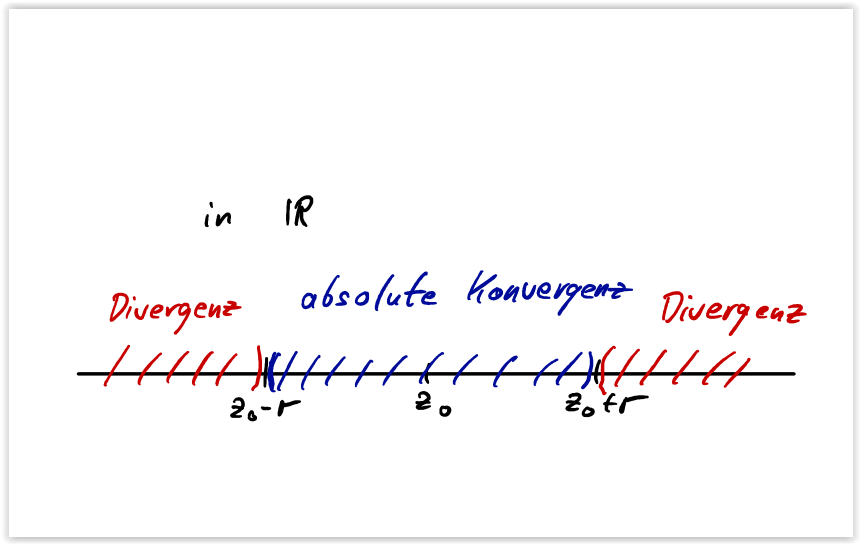
\includegraphics[width=0.8\linewidth]{./img/reihen_potenzreihen_r.png}
				  \caption{Potenzradius in $\R$ \protect\cite{HM12}}
				  \label{fig:reihe_potenzradius_r}
				\end{minipage}%
				\begin{minipage}{.5\textwidth}
				  \centering
				  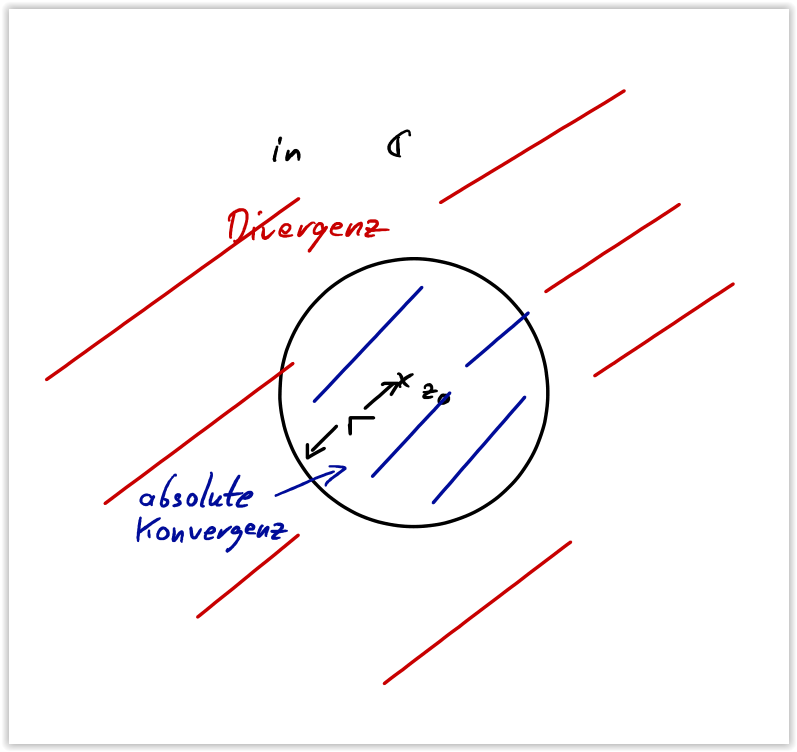
\includegraphics[width=0.55\linewidth]{./img/reihen_potenzreihen_c.png}
				  \caption{Potenzradius in $\C$ \protect\cite{HM12}}
				  \label{fig:reihe_potenzradius_c}
				\end{minipage}
      \end{figure}
	  \end{satz}
    \begin{bem}
      Falls einer der folgenden Grenzwerte existiert bzw. $\infty$ ist, ist er gleich dem Konvergenzradius.
      \begin{equation*}
        r = \frac{1}{\lim |a_k|^\frac{1}{k}} \quad bzw. \quad r = \lim\limits_{k \rightarrow \infty} \left| \frac{a_k}{a_{k+1}}\right|
      \end{equation*}
    \end{bem}	  
    \begin{bem}
      Da absolute Konvergenz vorliegt, können Potenzreiuhen miteinander multipliziert werden. Der Konvergenzradius ist mindestens so groß wie das Minimum der Konvergenzradien.
    \end{bem}
	  \begin{bem}
	    Potenzreihen sind innerhalb ihres Konvergenzradius beliebig oft diffbar und können gliedweise abgeleitet werden.
	  \end{bem}
	  \begin{satz}
	    Die formal abgeleitete Reihe $\sum\limits_{k = 1}^\infty a_k kx^{k-1}$ hat den gleichen Konvergenzradius wie die Ausgangsreihe.
	  \end{satz}
	  \begin{satz}
	    Es sei $\sum\limits_{k=0}\infty a_k x^k$ eine Potenzreihe mit Konvergenzradius $1$. Ist die Reihe auch in $x = 1$ konvergent, d.h. konvergiert $\sum\limits_{k = 0}^\infty$, so gilt
	    \begin{equation}
	      \lim\limits_{x\rightarrow 1} \sum\limits_{k = 0}^\infty a_k x^k = \sum\limits_ {k = 0}^\infty a_k
	    \end{equation}
	  \end{satz}
\newpage	  
	  